%!TEX root = doc.tex
\section{Related Work} % (fold)
\label{sec:related_work}

Some works have approaches the problem of complementing Repast and JADE's faults by bringing them together in a single framework by means of a middleware. In MISIA \cite{garcia2011misia} and JRep \cite{gormer2011jrep}, the authors' approach was successful in solving the needs of JADE in creating multi-agent-based simulations (MABS) by directly using the Repast framework and its rich simulation tools.

MISIA's approach to the integration of Repast and JADE, as suggested in figure \ref{fig:misia}, is to use a middle layer that acts as the bridge betweens the two layers which interface both frameworks. MISIA extends the representation of Repast and JADE agents and then allows them to communicate internally and to synchronize their state. Since JADE is event-driven, a coordinator informs the JADE-Agent when a tick has passed. On the other hand, Repast lacks native support to FIPA interaction protocols; MISIA introduces it's own implementation of these to enable them on Repast.

The main challenge when implementing the FIPA interaction protocols is to synchronize them with Repast tick-based simulation, since JADE is mostly event-driven. In MISIA, the implementation of these protocols deal with the notion of time by creating handlers that the programmer can re-implement when sending and receiving messages. All the tick handling is done behind the scenes.

\begin{figure}[h]
	\centering
	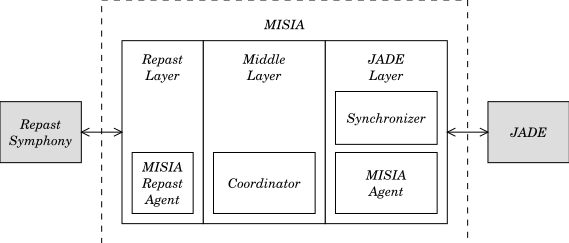
\includegraphics[width=0.5\textwidth]{figures/MISIA.png}
	\caption{Basic structure of MISIA}
	\label{fig:misia}
\end{figure}

JReps's approach is simpler than MISIA's. By placing the JADE agent representation inside the Repast agent, the synchronization is immediate. Each agent then takes care of interfacing their respective frameworks. The interaction between agents in JRep is performed with FIPA ACL; the protocols' implementation is provided by the JADE platform.

\begin{figure}[h]
	\centering
	\includegraphics[width=0.5\textwidth]{figures/jrep.png}
	\caption{Basic structure of JRep}
	\label{fig:jrep}
\end{figure}

The most obvious advantage of the approach proposed in this paper if the possibility of using Repast interaction protocols without the need to interface with JADE. JADE is a very rich platform, but for many simulation scenarios, the overhead introduce by it will have an impact on the simulation performance. The proposed API uses an implementation those protocols that is conceptually very close to JADE's but tailored for Repast with no extra dependencies - in fact, the API could be used with other frameworks with little to no adaptation.

Similar to MISIA, this API proposes an implementation of the protocols following JADE's. The programmer only have to register all behaviors in the appropriate Repast Simphony context, which deals with all the scheduling, and define the schedule interval and starting tick.

\begin{figure}[h]
	\centering
	\includegraphics[width=0.5\textwidth]{figures/repacl.png}
	\caption{Basic structure of RepACL API}
	\label{fig:relate-repacl}
\end{figure}